\documentclass{mprop}
\usepackage{graphicx}
\usepackage{amsthm}
\theoremstyle{definition}
\usepackage{mathtools}
\usepackage[numbers]{natbib}
\usepackage{thmtools}
\usepackage[usenames, dvipsnames]{color}
\usepackage{algorithm}
\usepackage{algpseudocode}
\usepackage{hyperref}
\usepackage{caption}
\usepackage{subcaption}

\newtheorem{example}{Example}
\newtheorem{theorem}{Theorem}

\declaretheoremstyle[headfont=\bfseries]{solution}
\declaretheoremstyle[headfont=\normalfont]{normalhead}
\declaretheorem[style=normalhead, numbered=no]{question}
\declaretheorem[style=normalhead, numbered=no]{instance}
\declaretheorem[style=solution, numbered=no]{solution}

% alternative font if you prefer
%\usepackage{times}

% for alternative page numbering use the following package
% and see documentation for commands
%\usepackage{fancyheadings}


% other potentially useful packages
%\uspackage{amssymb,amsmath}
%\usepackage{url}
%\usepackage{fancyvrb}
%\usepackage[final]{pdfpages}

\begin{document}

%%%%%%%%%%%%%%%%%%%%%%%%%%%%%%%%%%%%%%%%%%%%%%%%%%%%%%%%%%%%%%%%%%%
\title{The Traveller's Problem}
\author{Iva Stefanova Babukova}
\date{18 December 2016}
\maketitle
%%%%%%%%%%%%%%%%%%%%%%%%%%%%%%%%%%%%%%%%%%%%%%%%%%%%%%%%%%%%%%%%%%%

%%%%%%%%%%%%%%%%%%%%%%%%%%%%%%%%%%%%%%%%%%%%%%%%%%%%%%%%%%%%%%%%%%%
\tableofcontents
\newpage
%%%%%%%%%%%%%%%%%%%%%%%%%%%%%%%%%%%%%%%%%%%%%%%%%%%%%%%%%%%%%%%%%%%

%%%%%%%%%%%%%%%%%%%%%%%%%%%%%%%%%%%%%%%%%%%%%%%%%%%%%%%%%%%%%%%%%%%
\section{Introduction}\label{intro}

In this work we present the Traveller's Problem (TP), a computational task whose extensions and variations are often encountered by travellers around the world. The task is concerned with creating a valid travel schedule, using airplanes as a means of transportation and in accordance with certain constraints specified by the traveller.

%%%%%%%%%%%%%%%%%%%%%%%%%%%%%%%%%%%%%%%%%%%%%%%%%%%%%%%%%%%%%%%%%%%
\section{Problem Formulation}

Each instance of TP consists of:

\begin{enumerate}
\item A set of airports $A = \{ A_{0},...,A_{n} \}$ for $n > 0$. Each airport $A_{i}$ $\in$ $A$ represents a location the traveller can begin their commute in, visit as a desired destination, or connect in on the way to their destination.

\item The trip starts and ends at the same airport $A_{0}$, which is referred to as the \textit{home point}.

\item The total travel time $T$, within which the traveller must have visited all destinations and returned to the home point.
 
\item A set of flights $F = \{ f_{0},...,f_{m} \}$. Each flight $f_{j}$ has:
\begin{itemize}
\item departure airport $A^{d}_{j}$,
\item arrival airport $A^{a}_{j}$,
\item date $t_{j}$,
\item duration $\Delta_{j}$,
\item cost $c_{j}$,
\end{itemize} 
for some non-negative integer $j$ less than or equal to $n$.
The date $t_{j}$ is a positive rational number less than or equal to $T$ that shows at which day $f_{j}$ leaves its departure airport. The duration $\Delta{j}$ is a positive fraction that shows the amount of time that takes for flight $f_{j}$ to go from $A^{d}_{j}$ to $A^{a}_{j}$. The cost $c_{j}$ is a positive number that denotes the number of units of some currency $\epsilon$ that the traveller pays in order to be able to board flight $f_{j}$.

\item \textcolor{red}{Each airport $A_{i}$ has a \textit{connection time} $C_{A_{i}}$, that is the time that takes to switch from any flight $f_{p}$ with $A^{a}_{p} = A_{i}$ to any flight $f_{q}$ with $A^{d}_{q} = A_{i}$.}

\item A set of \textit{destinations} $D = \{ D_{1},...,D_{l} \}$, $D \subseteq A$, $l \leq n$.
\end{enumerate}

A solution to any instance of TP is a sequence $s$ of $k$ valid flights, $ \langle f_{i_{1}}, f_{i_{2}},...,f_{i_{k}} \rangle \\ \subseteq F$. We say that $s$ is valid if the flights in $s$ have the following properties:

\begin{enumerate}
\item $A^{d}_{i_{1}} = A^{a}_{i_{k}} = A_{0}$
\item $ A^{a}_{i_{j}} = A^{d}_{i_{j+1}},  \quad 0 < j < k  \quad j$
\item $ t_{i_{j}} + \Delta_{i_{j}} + C_{r} \leq t_{i_{j+1}}, \quad 0 < j \leq k, \quad \textrm{where } r = A^{d}_{i_{j+1}}$
% david mentioned about possibly adding this as a hard constraint?
\item $t_{i_{k}} + \Delta_{i_{k}} \leq T$
\item $ \forall D_{p} \in D, \textrm{ } \exists \textrm{ } f_{i_{j}} \in s \textrm{, such that } A^{a}_{i_{j}} = D_{p} $
\end{enumerate}

Note that a valid sequence of flights may contain one or more flights to and from airports that are not destinations. Such airports are called \textit{connections}.

% these statements are only really meaningful when you relate TP to TSP and also to VRP.
% \textcolor{red}{Also note that the current problem formulation accepts asymmetric flight costs, i.e. one might have two flights $f_{i}$ and $f_{j}$ such that $A^{d}_{i} = A^{a}_{j}$ and $A^{a}_{i} = A^{d}_{j}$. That does not imply that $c_{i} = c_{j}$. Moreover, the problem formulation does not restrict the flight cost to depend on the flight duration. Consequently, this implies that TP is \textit{asymmetric} and in general the flight cost need not satisfy the \textit{triangle inequality}.}

The \textit{optimization} version of TP (TPO) asks for an \textit{optimal} solution \textcolor{red}{$s$} which minimizes the total sum of the prices of the flights in $s$, denoted by $c(s)$.

The \textit{decision} version of TP (TPD) asks whether there exists a valid sequence of flights $s$, such that $c(s)$ is less than or equal to some given integer $B$. The solution of this problem is a `yes' or `no' answer.

There exist a variety of additional constraints and extensions that can be added to TP. Our problem formulation has only presented the hard constraints which every valid solution to a TP instance must satisfy. In real-world problems, travellers may have additional preferences (soft constraints) and requirements (hard constraints) with regards to their travel. These are discussed in the next two sections.

\subsection{Hard Constraints}
This section presents some additional constraints that might be imposed on a TP instance. If any of them is required, then a solution that does not satisfy the requirement is considered as invalid.

\begin{itemize}
\item Travellers may wish to spend a certain amount of days at a given destination, specified by both upper and lower bounds. The days may additionally be constrained to be consecutive or not.

\item Travellers may require to spend a given date at a given destination, for example due to an event occurring on that date in this destination.

\item Travellers may require not to fly through a given airport more than once.
\end{itemize}

\subsection{Soft Constraints}
It may be desirable to search for a solution that satisfies some of the following requirements:

\begin{itemize}
\item Travellers may wish to spend a certain amount $\delta_{i}$ of days in each destination $D_{i}$, where $\delta_{i}$ may be specified as a lower or an upper bound.

\item Travellers may wish to avoid taking connection flights. In such requirement, we wish to maximise the number of flights to and from destinations.

\item Travellers may want to spend as little time on flying as possible. In such case, we wish to find a solution that minimises the sum of the durations of all flights.
\end{itemize}

%% mention the problem with lexicographic optimisation and multi-objective opimisation
Note that we may have an instance for which all soft constraints can not be satisfied simultaneously. In such case, the traveller may be required to rank his requirements in an order of preference. The instance becomes a lexicographic optimisation problem, where
\textcolor{red}{we first optimise the highest ranked objective, and subject to this we optimise the second ranked objective and so on.}
If all requirements are equally important for the traveller, we have to solve a multiobjective optimisation problem, where the objectives are all constraints required by the traveller. Each of the objectives is given a weight of importance. The problem is then to optimize the objective function, composed by the constraints, each of them multiplied by its weight. Multiobjective and lexicographic optimisation problems are discussed later in this work. %% TODO: discuss them

Note that most of the aforementioned constraints can be viewed as either hard or soft, depending on the user requirements. It is therefore suggested that any attempt at an investigation of TP assumes as an additional non-functional requirement that any proposed model to solve TP is flexible and can be easily extended by adding, removing and modifying the aforementioned constraints.

\section{Worked Examples}
We present an example instance of TP and comment on some of its solutions.

\begin{example}
\label{example1}
A traveller wishes to visit 4 airports from a set of 7 airports available to travel to and from: 

Glasgow (G), Berlin (B), Milan (M), Amsterdam (A), Paris (P), Frankfurt (F), London (L).

Airport G is the home point, F and L are connections, and B, M, A and P are the destinations. The travel time of the traveller is 15 days. All available flights are listed on Table \ref{table:flights}. For simplicity, the duration of each flight is assumed to be 1 day. This means that if the traveller gets a flight at date $x$, they will reach the arrival airport at day $x+1$.

\begin{table}
\centering
\renewcommand{\arraystretch}{1.4}% Spread rows out...
\begin{tabular}{|l|c|c|c|c|c|}
\hline
\textbf{Flight No} & \textbf{Departs} & \textbf{Arrives} & \textbf{Date} & \textbf{Price} \\
\hline
GA1 & G & A & \date{1} & 74 \\
\hline
GF1 & G & F & \date{1} & 86 \\
\hline
FB2 & F & B & \date{2} & 156 \\
\hline
GL3 & G & L & \date{3} & 25 \\
\hline
MF3 & M & F & \date{3} & 78 \\
\hline
BP4 & B & P & \date{4} & 67 \\
\hline
AP4 & A & P & \date{4} & 58 \\
\hline
PM6 & P & M & \date{6} & 71 \\
\hline
FM8 & F & M & \date{8} & 234 \\
\hline
MF9 & M & F & \date{9} & 39 \\
\hline
FA10 & F & A & \date{10} & 220 \\
\hline
FB11 & F & B & \date{11} & 122 \\
\hline
FM12 & F & M & \date{12} & 250 \\
\hline
PL12 & P & L & \date{12} & 45 \\
\hline
BG13 & B & G & \date{13} & 335 \\
\hline
BL13 & B & L & \date{13} & 102 \\
\hline
AG13 & A & G & \date{13} & 90 \\
\hline
LG14 & L & G & \date{14} & 24 \\
\hline
\end{tabular}
\caption{List of flights with departure and arrival airports, flight date and price.}
\label{table:flights}
\end{table}
\end{example}

\begin{solution}
A valid solution of the TP instance in the example above is the sequence of flights $s$, where the each flight is represented by its flight number, specified in the first column of Table \ref{table:flights}:

$$ s = \langle GA1, AP4, PM6, MF9, FB11, BG13\rangle $$

The total flights cost $c(s)$ is 699.

A valid solution with lower cost is the following sequence:

$$ s^{\prime} = \langle GA1, AP4, PM6, MF9, FB11, BL13, LG14\rangle $$

Here $c(s^{\prime})$ is 483 and hence $s$ is not optimal.
\end{solution}

\begin{example}
\label{example2}
Given the same problem instance as in Example \ref{example1}, suppose that the traveller has booked a ticket for a concert in B on day 3. The traveller requires to attend the concert.
\end{example}

\begin{solution}
In such case, neither $s$, nor $s^{\prime}$ from Example \ref{example1} are solutions, because both of them assign the traveller to be at a different location (airport A) at day 3. The following sequence is a solution:

$$ s^{\prime\prime} = \langle GF1, FB2, BP4, PM6, MF9, FA10, AG13\rangle $$

The total cost $c(s^{\prime\prime})$ is equal to 729, which is more expensive than $s$ and $s^{\prime}$.
\end{solution}

\section{List of Problems}
\label{npcompleteproblems}

\textcolor{red}{This Section gives a list of known problems, referred to in this work when proving the NP-hardness of TP (Section \ref{npcompleteproof}) and when reviewing the existing work (Section \ref{sec:existingwork}). The problems, marked with an asterisk ($\ast$) next to their title, are known to be NP-complete \citep{thebible}.}

\begin{enumerate}

\item \textbf{Vehicle-Routing Problem \textsuperscript{*} (VRP)}
\begin{instance}
.
\end{instance}
\begin{question}
.
\end{question}

\item \textbf{Travelling Salesman Problem \textsuperscript{*} (TSP) \footnote{Note that TSP is a special case of VRP when only one vehicle is allowed.}}
\begin{instance}
Set $A$ of $n$ cities, distance $d(A_{i}, A_{j})$ between each pair of cities $A_{i}$, $A_{j}$ $\in$ $A$, positive integer $B$.
\end{instance}

\begin{question}
Is there a tour of $A$ having length $B$ or less, i.e., a permutation of cities $\gamma = \langle A_{\pi(1)}, A_{\pi(2)},...,A_{\pi(n)} \rangle $ of $A$ such that the total travel distance $L_{\gamma}$:
$$L_{\gamma} = \bigg( \sum_{i=1}^{n-1} d(A_{\pi(i)}, A_{\pi(i+1)}) \bigg) + d(A_{\pi(n)}, A_{\pi(1)}) \leq B \quad \textrm{?}$$
\end{question}

\item \textbf{Travelling Salesman Problem Under the Triangle Inequality\textsuperscript{*} (TSP-$\Delta$) \footnote{Note that this problem is a variant of TSP.}}
\begin{instance}
Set $A$ of $n$ cities, distance $d(A_{i}, A_{j})$ between each pair of cities $A_{i}$, $A_{j}$ $\in$ $A$ that satisfies the triangle inequality, positive integer $B$.
\end{instance}

\begin{question}
Is there a tour of $A$ having length $B$ or less, i.e., a permutation of cities $\gamma = \langle A_{\pi(1)}, A_{\pi(2)},...,A_{\pi(n)} \rangle $ of $A$ such that the total travel distance $L_{\gamma}$:
$$L_{\gamma} = \bigg( \sum_{i=1}^{n-1} d(A_{\pi(i)}, A_{\pi(i+1)}) \bigg) + d(A_{\pi(n)}, A_{\pi(1)}) \leq B \quad \textrm{?}$$
\end{question}

\item \textbf{Time-Constrained TSP\textsuperscript{*} (TCTSP) \footnote{Note that this problem is a variant of TSP.}}

\begin{instance}
Set $A$ of $n$ cities, distance d($A_{i}$, $A_{j}$) between each pair of cities $A_{i}$, $A_{j}$ $\in$ $A$, positive integer $B$, lower and upper bounds $l_{i}$ and $u_{i}$ respectively for each city $A_{i}$ that specify its time window.
\end{instance}

\begin{question}
\color{red}
Is there a permutation of cities $\gamma = \langle A_{\pi(1)}, A_{\pi(2)},...,A_{\pi(n)} \rangle$ of $A$, such that each city $A_{\pi_{j}}$ is visited at time $t_{j}$, where $l_{j} \leq t_{j} \leq u_{j}$, and 
$$L_{\gamma} = \bigg( \sum_{i=1}^{n-1} d(A_{\pi(i)}, A_{\pi(i+1)}) \bigg) + d(A_{\pi(n)}, A_{\pi(1)}) \leq B \quad \textrm{?}$$

\end{question}

\item \textbf{The Assignment Problem (AP)}

\begin{instance}
Set $A$ and set $B$ with equal size, cost $C(a,b)$ of matching $a \in A$ to $b \in B$.
\end{instance}

\begin{question}
Find a bijection $f: A \gets B$ such that $\sum_{a\in A} C(a,f(a))$ is minimised.
\end{question}
\item \textbf{Vehicle-Routing Problem (VRP)}
\item \textbf{Job-Shop Scheduling Problem (JSSP)}
\item \textbf{Longest Path Problem}
\end{enumerate}

%%%%%%%%%%%%%%%%%%%%%%%%%%%%%%%%%%%%%%%%%
\section{Complexity of TP}
We state a theorem about the complexity of TP and prove it.
\begin{theorem}
TPD is NP-complete.
\end{theorem}

\begin{proof}
\label{npcompleteproof}
This proof first shows the membership of TPD in the NP class of problems. Second, we prove the NP-hardness of TP by constructing a polynomial-time reduction from a known NP-complete problem $\Pi$ to TPD, where $\Pi$ is chosen to be TSP-$\Delta$, defined in Section \ref{npcompleteproblems}. Its NP-hardness follows by a reduction from the Hamiltonian Cycle problem. The proof is presented by \citet{thebible}.

Given an instance of TPD and $s$, which is a sequence of flights from $F$, we can write an algorithm that checks in polynomial time whether $s$ is a solution. To accept or reject validity, the algorithm only needs to traverse $s$ and check that it satisfies all required properties. Therefore, TP is in NP.

Let $\pi$ be an instance of TSP-$\Delta$. Let $\pi^{\prime}$ be an instance of TPD with the following properties:
\begin{itemize}
\item The set of airports in $\pi^{\prime}$ is identical to the set of cities in $\pi$ and it is similarly denoted as $A$ (a city in $\pi$ is called an airport in $\pi^{\prime}$). \textcolor{red}{Airport $A_{1}$ is the home point.}
\item Each airport in $A$ is also a destination.
\item The connection time $C_{A_{i}}$ for each airport $A_{i}$ is equal to 0.
\item $T$ is equal to \textcolor{red}{$n$ and the days start from 0.}
\item Let $C$ be the Cartesian product of the airports in $A$ with itself, that is $C = A \times A$ = \{($A_{i}, A_{j}$) : $A_{i}$ $\in$ $A$, $A_{j}$ $\in$ $A$, $i \neq j$\}. Then $F$ is a set of flights, such that for every ($A_{i}, A_{j}$) $\in$ $C$, there exists a flight $f_{k}$ in $F$, such that $A^{d}_{k} = A_{i}$ and $A^{a}_{k} = A_{j}$ for every date $0 \leq t < T$.
\item For every $f_{k}$ $\in$ $F$, $c_{k}$ is equal to $d(A^{d}_{k}, A^{a}_{k})$ in $\pi$. Therefore, the flight costs also satisfy the triangle inequality.
\item For every $f_{k}$ $\in$ $F$, $\Delta_{k}$ = 1.
\item $B$ is the upper bound on the allowed total cost.
\end{itemize}

%% TSP solution => also TP solution
\textcolor{red}{
Suppose that $\gamma$ = $ \langle A_{i_{1}}, A_{i_{2}},...,A_{i_{n}} \rangle $ is a solution to $\pi$, where $\langle i_{1},...,i_{n} \rangle$ is a permutation of $\langle 1,...,n \rangle $ and the total travel distance $L_{\gamma} \leq B$. In $\pi^{\prime}$, $\gamma$ is equivalent to the order of visited airports by some sequence of flights $s$ = $ \langle f_{j_{1}}, f_{j_{2}},...f_{j_{n}} \rangle $, such that for each $p$  $(1 \leq p \leq n)$ there exists $q$ $(1 \leq q \leq n)$ such that $A^{d}_{j_{q}} = A_{i_{p}}$ and $A^{a}_{j_{q}} = A_{i_{p+1}}$, where subscripts are taken modulo $n$. For each $q$ $(1 \leq q \leq n)$, $A^{a}_{j_{q}} = A^{d}_{j_{q+1}}$ and $t_{j_{q}} = q - 1$.}

\textcolor{red}{
Since $\gamma$ is a tour in $\pi$, $\gamma$ contains the home point in $\pi^{\prime}$ $A_{1}$ at some position $i_{p}$ $(1 \leq p \leq n)$, where subscripts are taken modulo $n$. Therefore, there exist flights $f_{j_{u}}$ and $f_{j_{v}}$ in $s$, with $A^{d}_{j_{u}} = A_{i_{p}}$ and $A^{a}_{j_{u}} = A_{i_{p+1}}$, and $A^{d}_{j_{v}} = A_{i_{p-1}}$ and $A^{a}_{j_{v}} = A_{i_{p}}$. Therefore, $A^{d}_{j_{u}} = A^{a}_{j_{v}} = A_{i_{p}}$ and $s$ satisfies the first property of a valid solution.}

\textcolor{red}{
From the construction of $s$, it follows that property 2 also holds. To satisfy property 3 and 4, it is sufficient to choose flights from $F$ such that for every $f_{j_{u}}$ $\in$ $s$, $t_{j_{u}}$ = $u-1$. We know that such flights exist in $F$ by the construction of the set $F$. Property 5 is satisfied, since all airports in $A$ are destinations.}

\textcolor{red}{
Since the cost of every flight in $F$ is equal to the distance between the two cities in $\pi$ that correspond to its departure and arrival airport, it follows that $c(s) = L_{\gamma} \leq B$.}

\textcolor{red}{
The sequence $s$ satisfies all requirements for a valid solution to $\pi^{\prime}$. Therefore, a solution of $\pi$ is also a solution to $\pi^{\prime}$.}

\textcolor{red}{
Conversely, suppose that $s = \langle f_{j_{1}},...,f_{j_{k}} \rangle $ is a solution to $\pi^{\prime}$, where the flights in $s$ visit destinations in the sequence $\gamma^{\prime}$ = $\langle A_{i_{1}}, A_{i_{2}},...,A_{i_{m}} \rangle$. We will prove that $\gamma^{\prime}$ is a solution of $\pi$.}

\textcolor{red}{
By construction of $\pi^{\prime}$, all $n$ airports in $A$ are also destinations. Therefore, $\gamma^{\prime}$ contains all cities in $A$, that is $m \geq n$. Suppose that $m > n$ and an arbitrary airport $A_{p}$ $(i_{1} \leq p < i_{n})$ is included more than once in $\gamma^{\prime}$. Then $s$ must contain one than one flight with arrival airport equal to $A_{p}$. 
The duration of each flight in $\pi^{\prime}$ is one day. Therefore, for every $q$ $(1 \leq q < n - 1)$, $t_{j_{q+1}} = q$. Since the traveller has only $n$ days of total travel time, $k = n$ and $s$ is restricted to contain exactly $n$ flights. The only way to visit $n$ destinations, given $n$ flights is that all flights in $s$ have unique arrival airports. Assuming that $A_{p}$ is visited more than once means that there is more than one flight with arrival airport equal to $A_{p}$, which is a contradiction. Therefore, $m = n$ and each airport in $A$ is visited exactly once.}

\textcolor{red}{
From the properties of $s$ it follows that $A^{d}_{j_{1}} = A^{a}_{j_{n}} = A_{1}$. Therefore, $\gamma^{\prime}$ is a cycle of size $n$. We know that $c(s) \leq B$. We assigned a cost of each flight $f_{k}$ in $F$ to be equal to $d(A^{d}_{k}, A^{a}_{k})$ in $\pi$. Therefore, the total travel distance $L_{\gamma^{\prime}} = c(s)$ which is less than or equal to $B$.}

\textcolor{red}{
According to the specifications of $\pi$, $\gamma^{\prime}$ is a solution. Therefore, a solution to $\pi^{\prime}$ is also a solution to $\pi$.}

The transformation from a TSP-$\Delta$ instance to an instance of TPD can be done in polynomial time. For each of the $n$($n$-1)/2 distances d($A_{i}$, $A_{j}$) that must be specified in $\pi$, it is sufficient to check that the same cost is assigned to the flights from $A_{i}$ to $A_{j}$ for all dates.

Therefore, TP is in NP and the decision version of TSP-$\Delta$ can be reduced to TPD in polynomial time, from which it follows that TPD is NP-complete.

\end{proof}

%%%%%%%%%%%%%%%%%%%%%%%%%%%%%%%%%%%%%%%%%%%%%%%%%%%%%%%%%%%%%%%%%%%
\section{Background Survey}

%present an overview of relevant previous work including articles, books, and existing software products. Critically evaluate the strengths and weaknesses of the previous work.

\label{sec:existingwork}
We present some existing approaches to dealing with NP-hard problems, namely branch and bound (Section \ref{branchandbound}), approximation algorithms (Section \ref{approxalgos}), constraint programming (Section \ref{cp}) and integer programming (Section \ref{ip}). \textcolor{red}{The way each of these methods tackles NP-hardness is illustrated with a specific NP-hard problem as an example, defined in Section \ref{npcompleteproblems}.}


\subsection{Integer Programming}
\label{ip}
% What is integer programming? (IP)
% What is an objective function?
Integer programming (IP) is a method for solving optimisation problems. Given an optimisation problem $\pi$ with a set of constraints $\zeta_{\pi}$ and a goal $G_{\pi}$, integer programming involves optimising $G_{\pi}$, subject to all constraints in $\zeta_{\pi}$, where $G_{\pi}$ is modeled as an expression, called an \textit{objective function} and the constraints in $\zeta_{\pi}$ are expressed as mathematical equations. All variables in the model are restricted to take only integer values. As an example of a problem, modeled and solved with IP, we give TSP.

% The polyhedral approach (\citet{Dantzig54} have made work on this)

% nonpolyhedral approximations that can be computed in polynomial-time, such as semidefinite relaxations

\subsubsection{Integer Programming Formulation of TSP}
% \texorpdfstring{TSP-$\Delta$}{Lg}}
\label{sec:iptspformulation}
We present the integer programming model for TSP and its variations, formulated by \citet{Dantzig54}.

Let $\pi$ be and instance of TSP. Let $x(i,j)$ be a variable that denotes whether the next city visited after $i$ is $j$ in some solution of $\pi$. The value of $x(i,j)$ is equal to 1 if this is true, or 0 if it is false. If $x(i,j)$ is 1, then $i$ is called the \textit{incoming} city and $j$ - the \textit{outgoing} city. One of the properties of a valid TSP tour is that each city is visited exactly once. This can be enforced with the following constraint:

\begin{equation}
\label{eq:one}
\begin{split}
  \sum_{j \in A} x(i,j) = 1, \qquad i \in A,\\
  \sum_{i \in A} x(i,j) = 1, \qquad j \in A,
\end{split}
\end{equation}

Constraint (\ref{eq:one}) ensures that each city in $A$ is picked exactly once as an incoming and an outgoing city. However, it allows for the existence of one or more cycles of $n_{1} < n$ cities, called \textit{subtours}. For instance, consider Figure \ref{fig:tour} and Figure \ref{fig:subtours}. Both of them satisfy constraint (\ref{eq:one}). However, Figure \ref{fig:subtours} does not represent a valid tour, because it contains two subtours, each of size 3. To tackle this problem, \citet{Dantzig54} introduce the \textit{subtour elimination} constraint, that is:

% \begin{equation}
% \label{eq:subtourElimination}
% \sum_{i\in S}\sum_{j\in S} x(i,j) \leq |S| - 1, \qquad \textrm{for all } S \subset V, S \neq \emptyset
% \end{equation}

\begin{equation}
\label{eq:subtourElimination}
\sum_{S\bar{S}} x(i,j) \geq 2, \qquad \textrm{for all } S \subset A, \bar{S} = A \setminus S, \quad \bar{S},S \neq \emptyset
\end{equation}

Here, $S$ is a set of cities, subset of A and $\bar{S}$ is the set of all cities that are in $A$ and not in $S$. Constraint (\ref{eq:subtourElimination}) enforces that at least two cities in $S$ are connected with cities from $\bar{S}$. We give Figure \ref{fig:tour} and Figure \ref{fig:subtours} as an example. Let $S = \{A_{1},A_{2},A_{3}\}$, then $\bar{S} = \{A_{4},A_{5},A_{6}\}$. Constraint (\ref{eq:subtourElimination}), would detect the tour on Figure \ref{fig:subtours} as invalid, as there is no city in $S$ that is connected to a city in $\bar{S}$. Figure \ref{fig:tour} will be accepted, since $A_{1}$ and $A_{3}$ are connected with $A_{6}$ and $A_{4}$ respectively. 

The objective function is:
\begin{equation}
\label{eq:two}
\sum_{i\in V}\sum_{j\in V} c(i,j)x(i,j)
\end{equation}

\begin{figure}
\centering
\begin{minipage}{.5\textwidth}
  \centering
  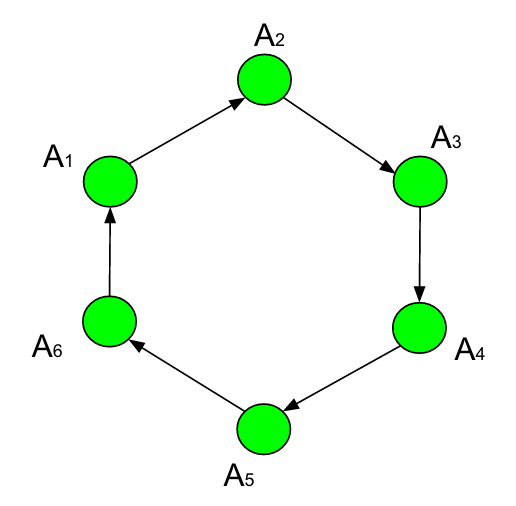
\includegraphics[width=4cm, height=4cm]{images/valid.png}
  \caption{A valid TSP tour}
  \label{fig:tour}
\end{minipage}%
\begin{minipage}{.5\textwidth}
  \centering
  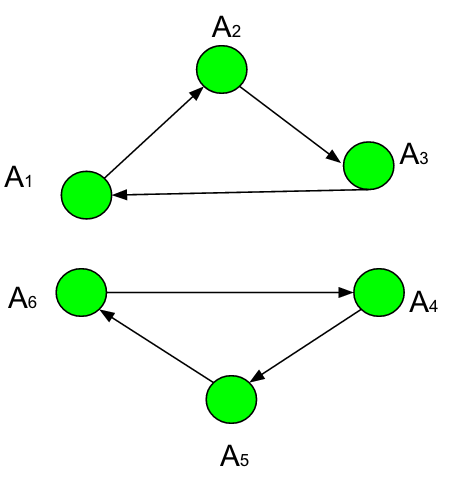
\includegraphics[width=4cm, height=4cm]{images/invalid.png}
  \caption{Two subtours of size 3}
  \label{fig:subtours}
\end{minipage}
\end{figure}

Equation (\ref{eq:two}) constrains that in a valid solution of $\pi$, each city has to be connected with exactly two cities. Note that formula (\ref{eq:two}) allows for solutions that include subtours, i.e. tours of length less than $n$. Equation (\ref{eq:subtourElimination}) is also known as \textit{subtour elimination} constraint and it serves the purpose to filter such invalid solutions.

In this formulation, one can remove constraint (\ref{eq:subtourElimination}) to obtain an instance of AP with the same cost function as $P$ \citep{Little63,Eastman58,Bellmore71}.

By dropping constraint (\ref{eq:subtourElimination}), the solution of $P_{AP}$ can be either a tour, or a collection of subtours. Hence, every tour of $P$ is a solution to AP, but not all solutions of AP are tours \citep{Bellmore71}. This allows for using the cost of the optimal solution of AP as a lower bound for the most optimal solution of $P$. In \cite{tspbible} it is showed with an experiment that both in theory and in practice the most optimal solution to AP is very likely to be a strong bound on $P$. The AP can be solved in at most $\mathcal{O}(n^{3})$ steps \citep{Kuhn55,Christofides75}. The ``bound'' procedure, that is called for every problem $P_{ij}$ in Algorithm \ref{alg:branchandbound}, computes AP$_{ij}$. It is shown in \cite{tspbible} that computing AP$_{ij}$ for each problem $P_{ij}$ in at most $\mathcal{O}(n^{2})$ steps by the Hungarian method \citep{Kuhn55}, provided that the algorithm is started from the optimal solution of the parent problem $P_{i}$.


\subsection{Branch and Bound Algorithms}
\label{branchandbound}
%% this is an enumerative method: The three most important enumerative methods are (i) implicit enumeration, (ii) dynamic programming, and (iii) branch and bound method
We present this technique for instances of TSP-$\Delta$. 
\textcolor{red}{
The origins of the branch and bound technique date back to the work by \citet{Dantzig54}, where an instance with 49 cities is solved and proved as optimal. The term ``branch and bound'' itself was introduced by \citet{Little63}.} 

\textcolor{red}{The branch and bound procedure repeatedly breaks up the set of feasible solutions into successively smaller subsets and calculates a \textit{bound} on the objective function value for each subset. The bounds are obtained by performing \textit{relaxation}, i.e. replacing the problem over a given subset with an easier (\textit{relaxed}) problem, such that the solution value of the latter bounds that of the former. Bounds are used to discard certain subsets from further consideration.}

\textcolor{red}{
Branch and bound procedure can be represented as a rooted tree whose root node corresponds to the original problem and the leafs of the tree form the set of all candidate solutions. The successor nodes of each non-leaf node $i$ correspond to the subproblems, defined by the branching rule.}

\textcolor{red}{
Algorithm \ref{alg:branchandbound} presents a pseudo code of the branch and bound technique. An active problem set $s$ is set to contain the problem set initially (line 3). Then, we branch on each problem $P_{i}$ chosen from $s$. The branching rule generates a set of subproblems $s_{i}$ (line 10). Each subproblem $P_{ij}$ in $s_{i}$ is then checked whether it is ``worse'' than the best one found so far by calculating its bound (line 12, 13). Problems with ``worse'' bounds are being discarded (line 14), otherwise they are added to $s$ for further investigation (line 19). If the current bound is the ``best'' found so far, its value is remembered and used for comparison with next problems. On termination, the algorithm returns the most optimal solution of $P$ (line 23).}

%% pseudocode for branch and bound procedure:
\begin{algorithm}
\color{red}
\centering
\caption{Branch and Bound Procedure}
\label{alg:branchandbound}
\begin{algorithmic}[1]
\Procedure{BB }{Problem $P$}
\State \textbf{begin}
\State s $\gets$ \{$P$\} \Comment{\textit{put $P$ in the list of active problems set s}}
\State bestVal $\gets$ NULL
\State currentBest $\gets$ NULL
\State currVal $\gets$ NULL
\While{s \textbf{not} $\emptyset$}
\State $P_{i}$ $\gets$ \Call{choose}{s} \Comment{\textit{choose next subproblem}}
\State s $\gets$ s - $P_{i}$
\State $s_{i}$ = \Call{branch}{$P_{i}$} \Comment{\textit{branch on $P_{i}$, returns a list of subproblems}}
\For{$P_{ij}$ in $s_{i}$}
\State currVal $\gets$ \Call{bound}{$P_{ij}$} \Comment{\textit{calculate the bound of $P_{ij}$}}
\If{currVal \textbf{worse than} bestVal}
\State kill $P_{ij}$ \Comment{\textit{$P_{ij}$ can not lead to an optimal solution}}
\ElsIf{$P_{ij}$ is a complete solution}
\State bestVal $\gets$ currVal
\State currentBest $\gets$ $P_{ij}$
\Else
\State s $\gets$ s + $P_{ij}$
\EndIf
\EndFor
\EndWhile
\State \Return{currentBest}
\EndProcedure
\end{algorithmic}
\end{algorithm}

\textcolor{red}{
Algorithm \ref{alg:branchandbound} does not tell much about the ``choose'', ``branch'' and ``bound'' procedures. This is because there are many variations of their implementations. We discuss some of them in the following parts of this section.}

\subsubsection{Bounds based on the Assignment Problem}
This relaxation is based on expressing the integer programming version of an optimisation problem $P$ as an assignment problem (AP) after dropping one or more constraints from $P$.
The AP relaxation is successfully used for solving TSP \cite{Little63,Eastman58,Bellmore71,tspbible,Baker83} and for the Vehicle Routing Problem (VRP) \citep{Laporte86,vrpbible}. We explain the principles of this relaxation using TSP as a use case.

% Let $P$ be an instance of TSP. The constraints of $P$ can be expressed with the following integer programming model \citep{tspbible,Dantzig54,Little63}:

% Let $G(V,E)$ be a complete directed graph with vertex set $V = \{1,...,n\}$, where each vertex corresponds to a city in $P$ and set of edges $E = \{(i,j) | i,j \in V\}$ and non-negative cost $c(i,j)$ for each edge $(i,j)$ that is equal to the distance $d(i,j)$ in $P$. For all $i \in V$, $c(i,i) = \infty$ and for all edges $(i,j)$ that one wishes not to include in a tour, $c(i,j) = \infty$. Let $x(i,j)$ be either 1, if edge $(i,j)$ is in the solution, or 0 otherwise. Then, following \cite{Dantzig54}, $P$ can be formulated as the problem of minimising

% \begin{equation}
% \label{eq:one}
% \sum_{i\in V}\sum_{j\in V} c(i,j)x(i,j)
% \end{equation}

% subject to

% \begin{equation}
% \label{eq:two}
% \begin{split}
%   \sum_{j \in V} x(i,j) = 1, \qquad i \in V,\\
%   \sum_{i \in V} x(i,j) = 1, \qquad j \in V,
% \end{split}
% \end{equation}

% \begin{equation}
% \label{eq:subtourElimination}
% \sum_{i\in S}\sum_{j\in S} x(i,j) \leq |S| - 1, \qquad \textrm{for all } S \subset V, S \neq \emptyset
% \end{equation}

% Equation (\ref{eq:two}) constrains that in a valid solution of $P$, each city has to be connected with exactly two cities. Note that formula (\ref{eq:two}) allows for solutions that include subtours, i.e. tours of length less than $n$. Equation (\ref{eq:subtourElimination}) is also known as \textit{subtour elimination} constraint and it serves the purpose to filter such invalid solutions.

% In this formulation, one can remove constraint (\ref{eq:subtourElimination}) to obtain an instance of AP with the same cost function as $P$ \citep{Little63,Eastman58,Bellmore71}.

% By dropping constraint (\ref{eq:subtourElimination}), the solution of $P_{AP}$ can be either a tour, or a collection of subtours. Hence, every tour of $P$ is a solution to AP, but not all solutions of AP are tours \citep{Bellmore71}. This allows for using the cost of the optimal solution of AP as a lower bound for the most optimal solution of $P$. In \cite{tspbible} it is showed with an experiment that both in theory and in practice the most optimal solution to AP is very likely to be a strong bound on $P$. The AP can be solved in at most $\mathcal{O}(n^{3})$ steps \citep{Kuhn55,Christofides75}. The ``bound'' procedure, that is called for every problem $P_{ij}$ in Algorithm \ref{alg:branchandbound}, computes AP$_{ij}$. It is shown in \cite{tspbible} that computing AP$_{ij}$ for each problem $P_{ij}$ in at most $\mathcal{O}(n^{2})$ steps by the Hungarian method \citep{Kuhn55}, provided that the algorithm is started from the optimal solution of the parent problem $P_{i}$.

%Performance

The AP relaxation is reported to perform differently, depending on the type of the problem \citep{tspbible,Bellmore71}. In particular, its performance highly depends on whether the problem has symmetric or asymmetric cost matrix. In the case with TSP, symmetric cost matrix refers to the property that the distance $d(i,j)$ from $i$ to $j$ is equal to $d(j,i)$. TSP with symmetric cost matrix is called Symmetric TSP (STSP) and Asymmetric TSP (ATSP) otherwise.

Experiments with ATSP instances have shown that the AP relaxation provides an excellent lower bound \citep{tspbible}. 

\subsubsection{Lagrangian relaxation}

\subsubsection{Choosing techniques}

\subsubsection{Branching rules}

% maybe remove this section
% \subsection{Dynamic Programming}
% \label{dynamicprogr}
% Use case: \cite{Christofides81}

\subsubsection{Performance of Branch and Bound Methods}
Until the late 1980s, the most effective exact approaches for the vehicle routing problem were mainly branch and bound algorithms \citep{vrpbible}.

\subsection{Approximation Algorithms}
\label{approxalgos}

\subsection{Constraint Programming}
\label{cp}
\subsubsection{Local Search}
\subsubsection{Heuristics}
\subsubsection{Use Case}
job-shop scheduling problem solution with CP

%%%%%%%%%%%%%%%%%%%%%%%%%%%%%%%%%%%%%%%%%%%%%%%%%%%%%%%%%%%%%%%%%%%
\section{Proposed Approach}

state how you propose to solve the software development problem. Show that your proposed approach is feasible, but identify any risks.

%%%%%%%%%%%%%%%%%%%%%%%%%%%%%%%%%%%%%%%%%%%%%%%%%%%%%%%%%%%%%%%%%%%
\section{Work Plan}

show how you plan to organize your work, identifying intermediate deliverables and dates.

%%%%%%%%%%%%%%%%%%%%%%%%%%%%%%%%%%%%%%%%%%%%%%%%%%%%%%%%%%%%%%%%%%%
% it is fine to change the bibliography style if you want
\bibliographystyle{plainnat}
\bibliography{mprop}
\end{document}
